\paragraph{Definition} En linje beskriven på formen $\begin{pmatrix}x\\y\\z\end{pmatrix}=P_{0}+t\bm{v}$ sägs vara på \underline{parameterform}.
Alltså är det \underline{linjens ekvation på parameterform} och t är parametern.

\paragraph{Ex} Bestäm en ekvation för den linje som går igenom $P=\begin{pmatrix}1\\1\\0\end{pmatrix}$ och $Q=\begin{pmatrix}0\\1\\1\end{pmatrix}$.
\subparagraph{Lösning} 
Vektorn $v=\overrightarrow{QP}=Q-P=\begin{pmatrix}1\\1\\0\end{pmatrix}-\begin{pmatrix}0\\1\\1\end{pmatrix}=\begin{pmatrix}1\\0\\-1\end{pmatrix}$\\
Linjen ges av: $\begin{pmatrix}y\\y\\z\end{pmatrix}=\begin{pmatrix}1\\1\\0\end{pmatrix}+t\begin{pmatrix}1\\0\\-1\end{pmatrix}=\begin{pmatrix}1+t\\1\\-t\end{pmatrix}$

\section{Linjer i planet}
Vi har 
Vi har sett att linjer i planet går att beskriva med en ekvation $Ax+By+C=0$.
Detta sägs vara \underline{linjens ekvation på normalform}.\\
Vektorn $\begin{pmatrix}0\\-C/B\end{pmatrix}-\begin{pmatrix}-C/A\\0\end{pmatrix}=\begin{pmatrix}C/A\\-C/B\\\end{pmatrix}$ är en riktningsvektor.\\
Men då är även $\frac{AB}{C}\begin{pmatrix}C/A\\-C/B\end{pmatrix}=\begin{pmatrix}B\\-A\end{pmatrix}$ är en riktningsvektor!\\
Vilket leder till att $\bm{n}=\begin{pmatrix}A\\B\end{pmatrix}$ en normal!
Varför? Jo, 
\begin{equation*}
    \begin{pmatrix}B\\-A\end{pmatrix}\cdot \begin{pmatrix}A\\B\end{pmatrix}=BA+(-A)B=0
\end{equation*}
En linje beskriven av ekvationen $Ax+By+C=0$ har $\bm{n}=\begin{pmatrix}A\\B\end{pmatrix}$ som en normal.
Vektorn $\begin{pmatrix}B\\A\end{pmatrix}$ är en riktningsvektor.

\paragraph{Ex} En linje ges av $\left\lbrace\begin{matrix}
    x=1+t\\y=3+2t
\end{matrix}\right\rbrace$.
Skriv linjen på normalform.
\subparagraph{Lösning} Vi vill bli av med t!\\
$t=1-x$ och $2t=y-3\Leftrightarrow t=\frac{y-3}{2}$\\
Alltså: $1-x=\frac{y-3}{2}\Leftrightarrow x+\frac{y}{2}-\frac{3}{2}-1=0\Leftrightarrow 2x+y-5=0$\\
Vi ser att $\begin{pmatrix}2\\1\end{pmatrix}$ är en normal!

\chapter{Plan i rummet}
Ett plan bestäms av en punkt och två icke-parallella vektorer som ligger i planet.
Ett plan kan dessutom bestämmas av en punkt samt en normalvektor.
Vi kan exempelvis välja $\bm{u}\times \bm{v}$ som normal.
\begin{center}
    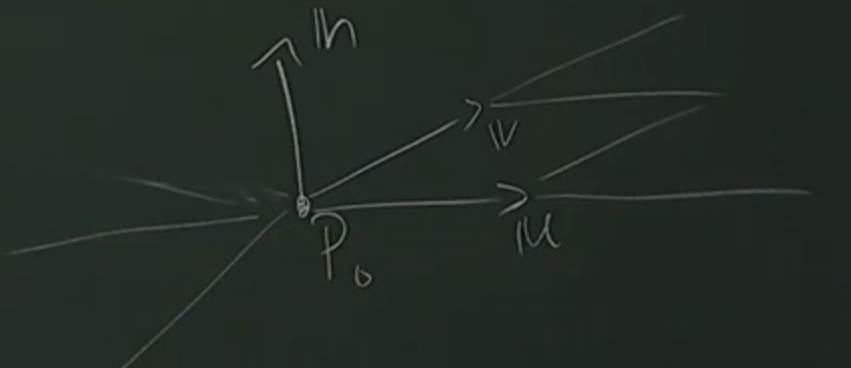
\includegraphics[scale=0.3]{imgs/img01.png}
\end{center}
Planets ekvation på parameterform: $
\begin{pmatrix}
    x\\y\\z
\end{pmatrix}
=
\begin{pmatrix}
    x_{0}\\y_{0}\\z_{0}
\end{pmatrix}
+s
\begin{pmatrix}
    u_{x}\\u_{y}\\u_{z}
\end{pmatrix}
+t
\begin{pmatrix}
    v_{x}\\v_{y}\\v_{z}
\end{pmatrix}$\\
Här är $s$, $t$ parametrar.\\
Antag att $\bm{n}=(A,B,C)$ är en normal till planet.
Då är $(x,y,z)$ en punkt planet $\Leftrightarrow \bm{n}\cdot \overrightarrow{P_{0}P}=0\Leftrightarrow \begin{pmatrix}
    A\\B\\C
\end{pmatrix}\cdot \begin{pmatrix}
    x-x_{0}\\y-y_{0}\\z-z_{0}
\end{pmatrix}=0\Leftrightarrow Ax+By+Cz-(Ax_{0}+By_{0}+Cz_{0})=0$\\
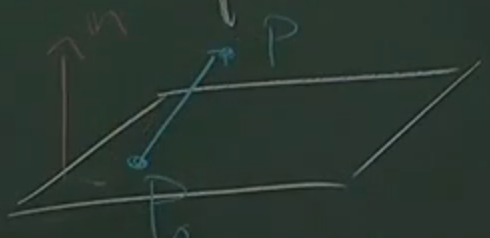
\includegraphics[scale=0.5]{imgs/img02.png}\\
Alltså: Planet ges av $Ax+By+Cz+D=0$ där $\bm{n}=(A,B,C)$ är en normal till planet!/?
Detta är planets ekvation på normalform!

\paragraph{Ex} Punkterna $P=\begin{pmatrix}
    1\\2\\3
\end{pmatrix}$, $Q=\begin{pmatrix}
    1\\4\\5
\end{pmatrix}$ och $R=\begin{pmatrix}
    3\\3\\8
\end{pmatrix}$ ligger på ett plan.
Skriv ner planets ekvation på parameterform och på normalform.
\subparagraph{Lösning} ~\\
$\bm{u}=\overrightarrow{PQ}=\overrightarrow{OQ}-\overrightarrow{OP}=\begin{pmatrix}
    0\\4\\5
\end{pmatrix}-\begin{pmatrix}
    1\\2\\3
\end{pmatrix}=\begin{pmatrix}
    -1\\2\\2
\end{pmatrix}$\\
$\bm{v}=\overrightarrow{PR}=\overrightarrow{OR}-\overrightarrow{OP}=\begin{pmatrix}
    3\\3\\8
\end{pmatrix}-\begin{pmatrix}
    1\\2\\3
\end{pmatrix}=\begin{pmatrix}
    2\\1\\5
\end{pmatrix}$\\
Planet på parameterform: $\begin{pmatrix}
    x\\y\\z
\end{pmatrix}=\begin{pmatrix}
    1\\2\\3
\end{pmatrix}+s\begin{pmatrix}
    -1\\2\\2
\end{pmatrix}+t\begin{pmatrix}
    2\\1\\5
\end{pmatrix} \Leftrightarrow \begin{Bmatrix}
    x=1-s+2t\\y=2+2s+t\\z=3+2d+5t
\end{Bmatrix}$\\
En normal ges ava $\bm{n}=\bm{u}\times \bm{v}=\begin{pmatrix}
    2\cdot 5-2\cdot 1\\
    2\cdot 2-(-1)\cdot 5\\
    (-1)\cdot 1-2\cdot 2
\end{pmatrix}=\begin{pmatrix}8\\9\\5\end{pmatrix}$\\
Planet ges av $8x=9y-5z+D=0$.
Punkten $p=\begin{pmatrix}1\\2\\3\end{pmatrix}$ liggger på planet!\\
$8\cdot 1+9\cdot 2-5\cdot 3+D=0\Leftrightarrow 26-15+D=0\Leftrightarrow D=15-26=-11$\\
Planets ekvation på normalform: $8x+9y-5z-11=0$

\section{Avstånd från en punkt till en linje}
Antag att vi har en linje L och en punkt P.
Tag R på linjen och låt Q vara den punkt på L som är närmast P.

Då är $\overrightarrow{RQ}=\overrightarrow{RP_{L}}$.  
$d=||\overrightarrow{RP}-\overrightarrow{RQ}||=||\overrightarrow{RP}-\overrightarrow{RP_{L}}||$    
% Bild 6

\paragraph{Ex} Beräkna avståndet från $P=\begin{pmatrix}1\\1\\1\end{pmatrix}$ 
till linjen L som ges av $\begin{pmatrix}
    x\\y\\z
\end{pmatrix}=\begin{pmatrix}
    1\\0\\0
\end{pmatrix}+t\begin{pmatrix}
    0\\1\\2
\end{pmatrix}$
\subparagraph{Lösning} Låt $R=\begin{pmatrix}
    1\\0\\0
\end{pmatrix}$.
$\overrightarrow{RP}=\overrightarrow{OP}-\overrightarrow{OR}=\begin{pmatrix}
    1\\1\\1
\end{pmatrix}-\begin{pmatrix}
    1\\0\\0
\end{pmatrix}=\begin{pmatrix}
    0\\1\\1
\end{pmatrix}$
% Bild 7
En riktningsvektor för linjen ör $\bm{v}=\begin{pmatrix}
    0\\1\\2
\end{pmatrix}$
Då är $\overrightarrow{RP_{L}}=\frac{\overrightarrow{RP}\cdot \bm{v}}{\bm{v}\cdot \bm{v}}\bm{v}=\frac{
    \begin{pmatrix}
        0\\1\\1
    \end{pmatrix}\cdot
    \begin{pmatrix}
        0\\1\\2
    \end{pmatrix}
}{
    \begin{pmatrix}
        0\\1\\2
    \end{pmatrix}\cdot
    \begin{pmatrix}
        0\\1\\2
    \end{pmatrix}
}\begin{pmatrix}
    0\\1\\2
\end{pmatrix}=\frac{1+2}{1+4}\begin{pmatrix}0\\1\\2\end{pmatrix}=\frac{3}{5}\begin{pmatrix}0\\1\\2\end{pmatrix}$
$d=||\overrightarrow{RP}-\overrightarrow{RP_{L}}||=||\begin{pmatrix}
    0\\1\\1
\end{pmatrix}-\frac{3}{5}+\begin{pmatrix}
    0\\1\\2
\end{pmatrix}||=||\begin{pmatrix}
    0\\\frac{2}{5}\\-\frac{1}{5}
\end{pmatrix}||=\sqrt{0^{2}+\frac{2}{5}^{2}+(-\frac{1}{5})^{2}}=\frac{1}{5}\sqrt{4+1}=\frac{\sqrt{5}}{5}$

\section{Avstånd från en punkt till ett plan}
Låt $\pi$ vara ett plan givet av $Ax+By+Cz+D=0$ och $P=\begin{pmatrix}x\\y\\z\end{pmatrix}$ någon punkt.\\
Tag $P_{0}=\begin{pmatrix}x_{0}\\y_{0}\\z_{0}\end{pmatrix}$ i planet.\\
N är en linje som är normal till $\pi$.
$d=||\overrightarrow{P_{0}P_{N}}||=\frac{||\overrightarrow{P_{0}P_{N}}\cdot \bm{n}||}{||\bm{n}||}=\frac{
    ||\begin{pmatrix}
        x-x_{0}\\y-y_{0}\\z-z_{0}
    \end{pmatrix}\cdot
    \begin{pmatrix}
        A\\B\\C
    \end{pmatrix}||
}{
    ||\begin{pmatrix}
        A\\B\\C
    \end{pmatrix}||
}$
% Bild 7 